%                      Code_Saturne version 1.3
%                      ------------------------
%
%     This file is part of the Code_Saturne Kernel, element of the
%     Code_Saturne CFD tool.
%
%     Copyright (C) 1998-2008 EDF S.A., France
%
%     contact: saturne-support@edf.fr
%
%     The Code_Saturne Kernel is free software; you can redistribute it
%     and/or modify it under the terms of the GNU General Public License
%     as published by the Free Software Foundation; either version 2 of
%     the License, or (at your option) any later version.
%
%     The Code_Saturne Kernel is distributed in the hope that it will be
%     useful, but WITHOUT ANY WARRANTY; without even the implied warranty
%     of MERCHANTABILITY or FITNESS FOR A PARTICULAR PURPOSE.  See the
%     GNU General Public License for more details.
%
%     You should have received a copy of the GNU General Public License
%     along with the Code_Saturne Kernel; if not, write to the
%     Free Software Foundation, Inc.,
%     51 Franklin St, Fifth Floor,
%     Boston, MA  02110-1301  USA
%
%-----------------------------------------------------------------------
\section{General}
%----------------

        \subsection{Objective}
%-----------------------------

The aim of this case is to train the user of \CS\ on a simplified but real 3D
computation. It corresponds to a stratified flow in a T-junction. The test case
will be used to present some advanced post-processing techniques.


        \subsection{Description of the configuration}
%-----------------------------------------------

The configuration is based on a real mock-up designed to characterize thermal
stratification phenomena and associated fluctuations. The geometry is shown on
figure \ref{config}.


\begin{figure}[h!]
\begin{center}
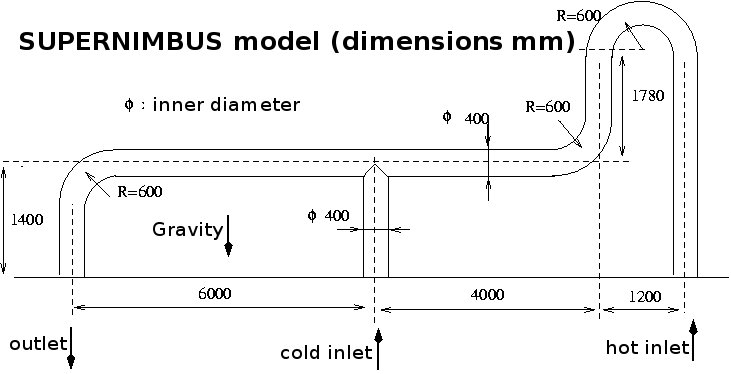
\includegraphics[width=9cm,height=4.5cm]{\repgraphics/c5_config.jpg}
\caption{Geometry of the case}
\label{config}
\end{center}
\end{figure}

There are two inlets, a hot one in the main pipe and a cold one in the vertical nozzle.
The volumic flow rate is identical in both inlets. It is chosen small enough so that
gravity effects are important with respect to inertia forces. Therefore
cold water creeps backwards from the nozzle towards the elbow until the flow
reaches a stable stratified state.


        \subsection{Characteristics}
%----------------------------------

Characteristics of the geometry: \\

\begin{center}
\begin{tabular}{|l|c|}
\hline
Diameter of the pipe & $D_{b} = 0.40\ m$ \\
\hline
\end{tabular}\\
\end{center}

Characteristics of flow:

\begin{center}
\begin{tabular}{|l|c|}
\hline
Cold branch volume flow rate & $Dv_{cb} = 4\ l.m^{-1}$ \\
\hline
Hot branch volume flow rate & $Dv_{hb} = 4\ l.m^{-1}$ \\
\hline
Cold branch temperature & $T_{cb} = 18.26$\degresC \\
\hline
Hot branch temperature & $T_{hb} = 38.5$\degresC \\
\hline
\end{tabular}\\
\end{center}

The initial water temperature in the domain is equal to 38.5\degresC.

Water specific heat and thermal conductivity are considered constant and
calculated at 18.26\degresC\ and $10^{5}\ Pa$:
\begin{itemize}
        \item heat capacity: $C_{p} = 4_,182.88\ J.kg^{-1}.\mbox{\degresC}^{-1}$
        \item thermal conductivity: $\lambda = 0.601498\ W.m^{-1}.\mbox{\degresC}^{-1}$
\end{itemize}

The water density and dynamic viscosity are variable with the temperature. The
functions are given below.


        \subsection{Mesh characteristics}
%---------------------------------------
The mesh used in the actual study had 125\,000 elements. It has been coarsened
for this example in order for calculations to run faster. The mesh used here
contains 16\,320 elements.

{\bfseries Type}: unstructured mesh

{\bfseries Coordinates system}: cartesian, origin on the middle of the horizontal pipe at the intersection with the nozzle.

{\bfseries Mesh generator used}: SIMAIL

{\bfseries Color definition}: see figure \ref{fige1_e5}.

\begin{figure}[h!]
\begin{center}
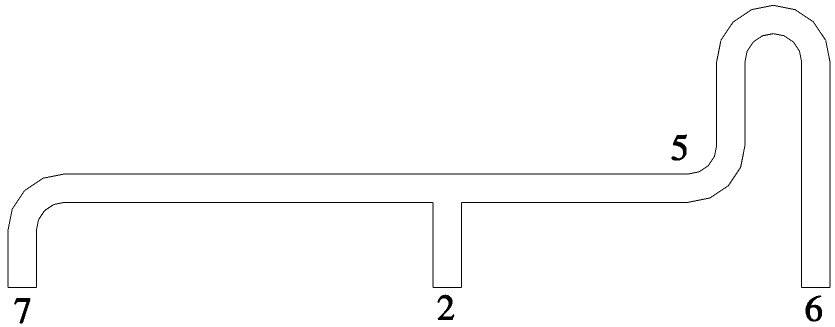
\includegraphics[width=10cm]{\repgraphics/color_Snimbus.jpg}
\caption{Colors of the boundary faces}
\label{fige1_e5}
\end{center}
\end{figure}


%-----------------------------
\section{CASE 5: Stratified junction}
%-----------------------------
In this case, advanced post-processing features will be used. A specific
pos-processing sub-mesh will be created, containing all the cells with a
temperature lower than 21\degresC, so that it can be visualized (with EnSight
for instance). The variable ``temperature'' will be post-processed on this
sub-mesh. A 2D clip plane will also be extracted along the symmetry plane of the
domain and temperature will be written on it.


        \subsection{Calculation options}
%-----------------------------------------

The following options are considered for the case:
\begin{itemize}
\renewcommand{\labelitemi}{$\rightarrow$}
        \item Flow type: unsteady flow
        \item Time step: variable in time and uniform in space
        \item Turbulence model: $k-\epsilon$
        \item Scalar(s): temperature
        \item Physical properties: uniform and constant for specific heat and
thermal conductivity and variable for density and dynamic viscosity
        \item Specific treatment of hydrostatic pressure: activated
        \item Time step limitation by gravity effects
\end{itemize}


        \subsection{Initial and boundary conditions}
%---------------------------------------------------

\begin{itemize}
\renewcommand{\labelitemi}{$\rightarrow$}
        \item Initialization: temperature initialization at 38.5\degresC
\end{itemize}

The boundary conditions are defined as follows:

\begin{itemize}
        \item {\bfseries Flow inlet}: Dirichlet condition
        \begin{itemize}
                \item velocity of $0.03183\ m.s^{-1}$ for both inlets
                \item temperature of 38.5\degresC\ for the hot inlet
                \item temperature of 18.6\degresC\ for the cold inlet
        \end{itemize}
        \item {\bfseries Outlet}: default value
        \item {\bfseries Walls}: default value
\end{itemize}

Figure \ref{fige1_e5} shows the colors used for boundary conditions and
table \ref{tabante51} defines the correspondance between the colors and
the type of boundary condition to use.

\begin{table}
\begin{center}
\begin{tabular}{|c|c|}
\hline
Colors & Conditions \\
\hline
2 & Cold inlet \\
\hline
6 & Hot inlet \\
\hline
7 & Outlet \\
\hline
5 & Wall \\
\hline
\end{tabular}
\caption{Boundary faces colors and associated references}
\label{tabante51}
\end{center}
\end{table}


        \subsection{Parameters}
%------------------------------
All the parameter necessary to this study can be defined through the Graphical
Interface, except the variable fluid characteristics and the advanced
post-processing features that have to be specified in user routines.


\begin{center}
\begin{tabular}{|l|c|}
\hline
\multicolumn{2}{|c|}{Parameters of calculation control} \\
\hline
Number of iterations & 100 \\
\hline
Reference time step & $1\ s $ \\
\hline
Maximal CFL number & 20 \\
\hline
Maximal Fourier number & 60 \\
\hline
Minimal time step & $0.01\ s$ \\
\hline
Maximal time step & $70\ s$ \\
\hline
Time step maximal variation & $0.1$ \\
\hline
Period of output chronological files & $10$ \\
\hline
\end{tabular}\\
\end{center}



        \subsection{Output management}
%-------------------------------------
The standard options for output management will be used. Four monitoring points
will be created at the following coordinates:

\begin{center}
\begin{tabular}{|c|c|c|c|}
\hline
Points & X(m) & Y(m) & Z(m)\\
\hline
1 & 0.010025 & 0.01534 & -0.011765 \\
\hline
2 & 1.625 & 0.01534 & -0.031652 \\
\hline
3 & 3.225 & 0.01534 & -0.031652 \\
\hline
4 & 3.8726 & 0.047481 & 7.25 \\
\hline
\end{tabular}
\end{center}



        \subsection{User routines}
%---------------------------------

The following routines have to be copied from the folder FORT/USER/base into the
folder FORT\footnote{only when they appear in the FORT directory will they be
taken into account by the code}: usphyv.F, usdpst.F, usvpst.F and usmpst.F


$\bullet$ {\bfseries usphyv.F}\\
This routine allows to specify variable physical properties, density and
viscosity in particular. In this case, the following variation laws are specified:
\begin{equation}
\rho = T.(A.T + B) + C
\end{equation}
where $\rho$ is the density, $T$ is the temperature, $A = -4.0668\times10^{-3}$,
$B =-5.0754\times 10^{-2}$ and $C = 1\,000.9$


For the dynamic viscosity, the variation law is:

\begin{equation}
\mu = T.(T.(AM.T + BM) + CM) + DM
\end{equation}
where $\mu$ is the dynamic viscosity, $T$ is the temperature,
$AM=-3.4016\times 10^{-9}$, $BM = 6.2332\times 10^{-7}$,
$CM = -4.5577\times 10^{-5}$ and $DM = 1.6935\times 10^{-3}$


\textbf{Note:} in the example routine, the examples are protected by a test to prevent any
undesired use. Do not forget to deactivate them.

In order for the variable density to have an effect on the flow, gravity must be
set to a non-zero value. $\vect{g} = -9.81 \vect{e}_y$ will be specified in the
Graphical Interface.


In this test case, advanced post-processing features will be used. A clip
plane will be created, along the symmetry plane of the domain, on which the
temperature will be written. This plane will be added to the standard
``writer'' ({\em i.e.} it will be an extra part in the standard CHR.ENSIGHT
case). The periodicity of output on the standard writer will be 10 iterations.\\
An additional writer will also be created, with a periodicity of 5
iterations. It will only contain one part ({\em i.e.} one sub-mesh): the set
cells where the temperature is lower than 21\degresC. The temperature will be
written on this part. The interest of this part is that it is time dependent
as for the cells it contains.

Three Fortran routines will be used:

$\bullet$ {\bfseries usdpst.F}\\
This routine is called only once, at the beginning of the calculation. It allows
to define the different writers and parts.

$\bullet$ {\bfseries usmpst.F}\\
This routine is called at each time step. It allows to redefine the content of
certain parts using any variable, especially the temperature for this case.

$\bullet$ {\bfseries usvpst.F}\\
This routine is called at each time step. It allows to specify which variable
will be written on which part.


        \subsection{Results}
%---------------------------

Figure \ref{fige2_e5} shows the evolution of the temperature in the domain at
different time steps. The evolution of the stratification is clearly visible.


\begin{figure}
\begin{center}
\begin{tabular}{c}
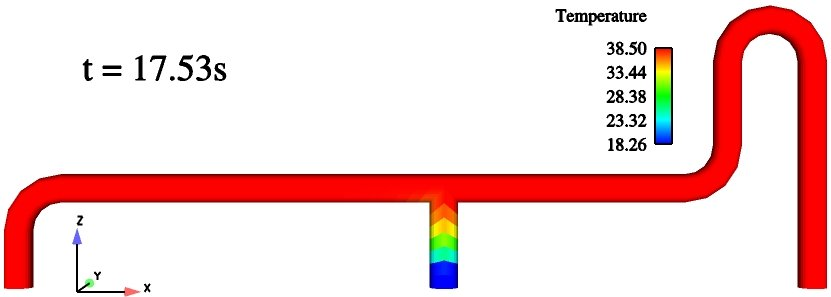
\includegraphics[width=10cm]{\repgraphics/case5_05.jpg} \\
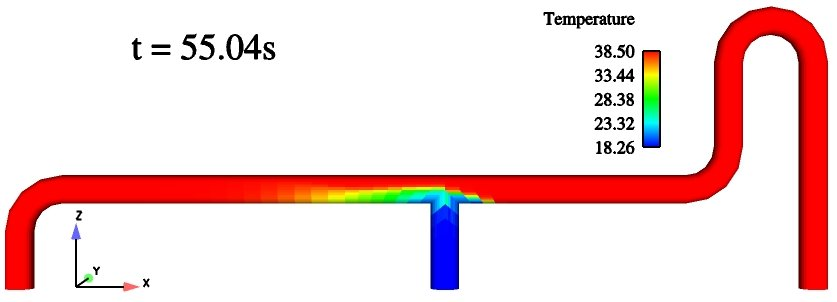
\includegraphics[width=10cm]{\repgraphics/case5_06.jpg} \\
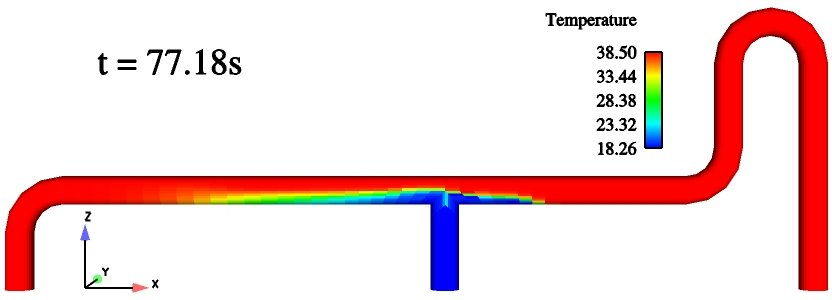
\includegraphics[width=10cm]{\repgraphics/case5_07.jpg} \\
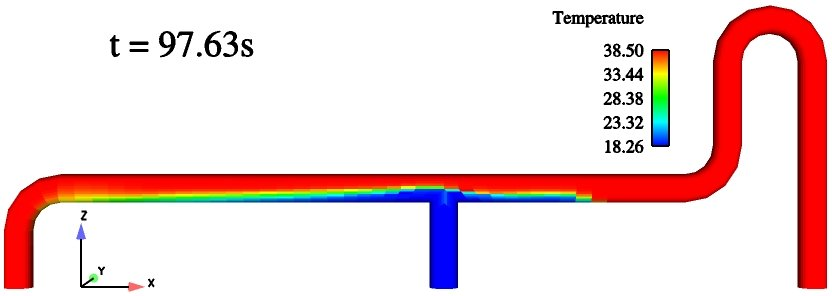
\includegraphics[width=10cm]{\repgraphics/case5_08.jpg} \\
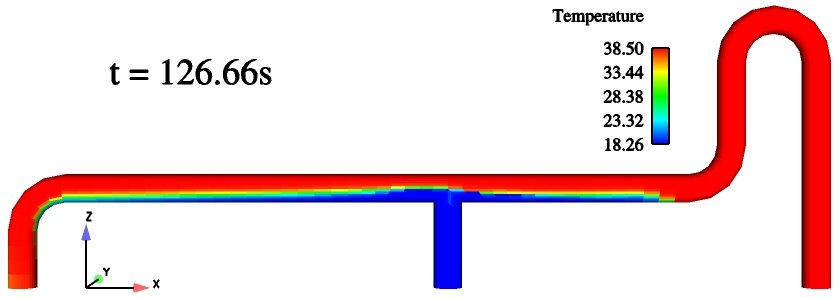
\includegraphics[width=10cm]{\repgraphics/case5_09.jpg} \\
\end{tabular}
\caption{Evolution of temperature}
\label{fige2_e5}
\end{center}
\end{figure}



Figure \ref{fige4_e5} shows the cells where the temperature
is lower than 21\degresC. It is not an isosurface created from the full domain,
but a visualization of the full sub-domain created through the post-processing
routines.

\begin{figure}[h!]
\begin{center}
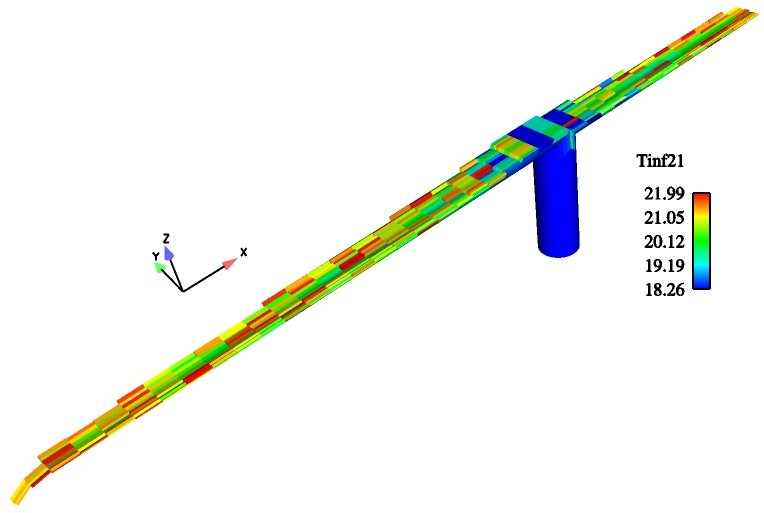
\includegraphics[width=10cm]{\repgraphics/case5_03.jpg}
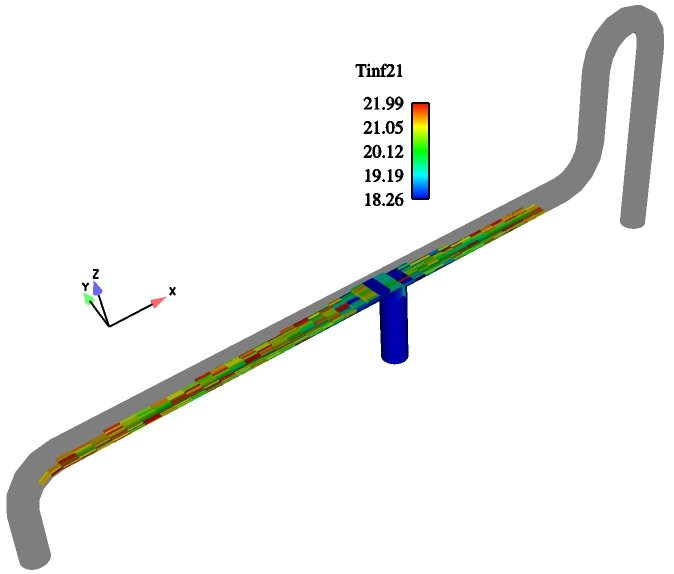
\includegraphics[width=10cm]{\repgraphics/case5_04.jpg}
\caption{Sub-domain where the temperature is lower than 21\degresC\ (upper figure)
and localization in the full domain (lower figure)}
\label{fige4_e5}
\end{center}
\end{figure}
